\section{Execution Schedules of Reconfigurable Architectures} 
\begin{figure*}
\begin{subfigure}[b]{0.34\textwidth}
\inputminted{python}{code/spatialeg2.py}
\caption {
}
\end{subfigure}
\hfill
\begin{subfigure}[b]{0.65\textwidth}
\centering
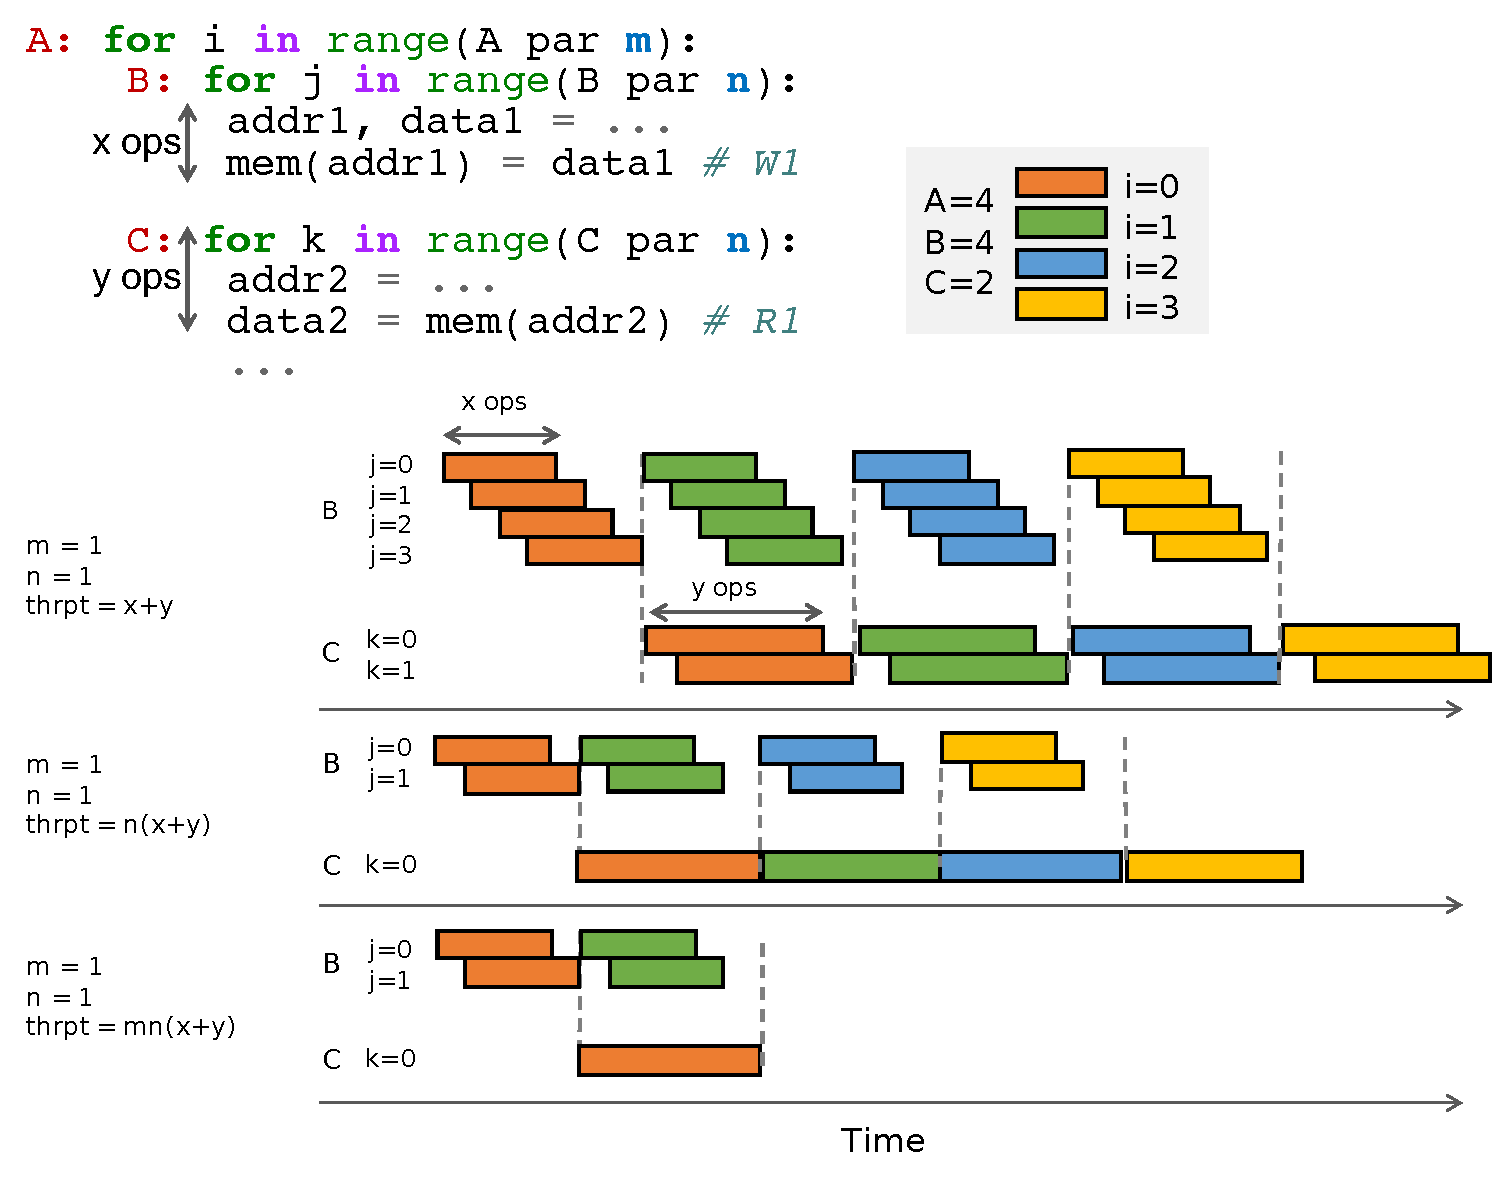
\includegraphics[width=1.0\textwidth]{figs/pipeexec.pdf}
\caption {
}
\end{subfigure}
\caption[Hiearchical pipelining and parallelization on spatial architecture]{
Hierarchical pipelining and parallelization in spatial architecture.
(a) illustrates the runtime and throughput of a hierarchically pipelined and parallelized program on
a reconfigurable spatial architecture. 
At the inner level, instructions within each basic
block are fine-grained pipelined across iterations of the innermost loop. 
At the outer level, the inner loops are coarse-grained pipelined across the outer loop iterations.
Exploiting multiple levels of pipeline parallelism gives a total throughput of $x+y$ operations per
  cycle, where \emph{x} and \emph{y} are number of operations in the basic blocks.
(b) Vectorizing the inner most loops B and C by \texttt{n} increases the throughput to $(x+y)n$.
(c) Parallelizing the outer loop A by \texttt{m} further increases the throughput to $(x+y)mn$.
}
\label{fig:pipeexec}
\end{figure*}

The key advantage of reconfigurable spatial accelerators, compared to processor-based architectures, 
is the ability to explore multiple levels of pipeline parallelism. 
In traditional Von Neumann architectures~\cite{vonneumann}, like CPUs and GPUs,
a computer consists of a processing unit that performs
computation, a memory unit that stores the program states, and a control unit that tracks execution states and fetches the instruction to execute. This computing model inherently assumes that
instructions within a program are executed in time, maximizing the flexibility to context switching between different workloads dynamically.

Reconfigurable accelerators are a direct violation of the von Neumann execution model; 
instructions are statically embedded in the datapath and executed in space as supposed to in time.
One of the disadvantages of reconfigurable hardware is paying the resource cost for infrequently
executed instructions, making it unsuitable for control-heavy workloads that traditional
processors are efficient at.
On the other hand, RDAs are particularly competitive in providing high-throughput, 
low-latency, and energy-efficiency acceleration for data-analytical workloads.
Data-analytical workloads encompass wide domains of applications, including image processing,
recognition, machine translation, digital signal processing, network processing, etc.
These applications exhibit a rich amount of data-level parallelism with relatively static control
flow.

\Cref{fig:pipeexec} shows an example of hierarchical parallelism and pipelining exploit by
a spatial architecture.
The overall compute throughput of a parallelized and pipelined program is 
the product of the total parallelization factors and pipelining depth.
By exploring multiple dimensions of concurrency in the program, spatial architecture is more likely
to achieve a good compute throughput for a wide range of applications.
For applications that are expensive to parallelize due to irregular access patterns, spatial
architectures can increase on the pipelining dimension;
for application with embarrassingly parallel workloads, spatial architecture can budget most
resource on increasing parallelism.

Another benefit of pipelined execution is that it is relatively easy to achieve good memory performance.
Data accessed by different stages of the pipelines are stored in discrete scratchpads instead of a shared cache; improving the effective on-chip bandwidth and capacity.
Using explicitly managed scratchpad also tends to improve locality and eliminate cache performance issues, such as thrashing.
Across kernels, pipelined execution reduces the amount of off-chip accesses for intermediate
data.
SIMT architectures, like GPUs, relying on high-bandwidth DRAM technology, such as HBM, to sustain
the compute throughput of massively parallelized threads.
While providing over 10x more bandwidth than traditional DDR technologies, HBM is very limited in
capacity, around 16GB as supposed to on the orders of TB for DDR.
As a result, the limited off-chip capacity often restricts the type of applications that
GPUs can support.

%\begin{table*}
  %\centering
%\begin{tabular}{lccc}
  %\toprule
 %Concurrency Level & Instruction & Data & Task/Kernel  \\ \midrule
 %Parallelsim & CPU,\rda & CPU,GPU,\rda & CPU,\rda  \\
 %Pipelining & \rda & \rda & \rda \\
 %\bottomrule
%\end{tabular}
%\caption[Concurrency level explored by different architectures]{
  %Concurrency level explored by different architectures
%}
%\label{tab:conclevel}
%\end{table*}

